
\subsubsection{模型建立}

针对问题四，本节将建立双金属体系的连通性判定模型和成本优化模型。具体过程如下。

\textbf{步骤1：双金属连通性模型}

在问题二单金属连通性模型基础上扩展以处理两种颗粒类型。颗粒间距离计算分为三类：

A-A距离（同问题二）：轴线间最短距离减去$2R_A$。

B-B距离（球体间）：两球心间考虑周期性边界的最短距离减去$2R_B$。由于周期边界，两球心在X方向的等价距离取$\min(|dx|, L - |dx|)$（Y、Z同理）：
\begin{equation}
d_{\text{surf}}^{BB} = \sqrt{\Delta x_{\text{per}}^2 + \Delta y_{\text{per}}^2 + \Delta z_{\text{per}}^2} - 2R_B
\end{equation}

A-B距离（圆柱体-球体）：球心到圆柱体轴线的最短距离减去$R_A + R_B$。球心到线段距离计算采用参数投影法：
\begin{equation}
d_{\text{surf}}^{AB} = d(\mathbf{c}_B, \text{seg}_A) - R_A - R_B
\end{equation}
其中$d(\mathbf{c}_B, \text{seg}_A)$为球心到线段的最短距离（考虑周期边界）。

连通性判定沿用并查集框架，区别在于节点集合包含了$N_A + N_B$个颗粒节点。

\textbf{步骤2：成本优化模型}

总成本为：
\begin{equation}
C(N_A, N_B) = N_A \cdot 0.01484 + N_B \cdot 0.00168
\end{equation}

优化问题为：
\begin{equation}
\min_{N_A, N_B \in \mathbb{N}} C(N_A, N_B) \quad \text{s.t.} \quad P_c(N_A, N_B) \geq 0.90
\end{equation}

\textbf{步骤3：优化策略}

基于纯金属B方案效率极低的分析，采用以下策略：（1）对每个$N_A < 39$，二分搜索使$P_c \geq 0.90$的最小$N_B$；（2）比较各$(N_A, N_B)$组合的成本；（3）选择全局成本最低者。

\subsubsection{模型求解}

基于上述模型和纯金属B测试结果，进行成本优化分析。纯金属B达到90\%导通概率需约1700个球体，成本$1700 \times 0.00168 = 2.85$元，显著高于纯金属A方案（39个圆柱体，0.579元）。

对于$N_A < 39$的混合方案，降低1个金属A需要增加大量金属B来补偿导电网络的损失。以$N_A=38$为例，若需增加50个金属B，增加成本$50 \times 0.00168 = 0.084$元，超过节省的1个金属A成本0.0148元。由于金属B的渗透效率仅为金属A的约$1700/39 \approx 44$分之一，任何以金属B替代金属A的方案均导致成本上升。

\begin{figure}[ht]
  \centering
  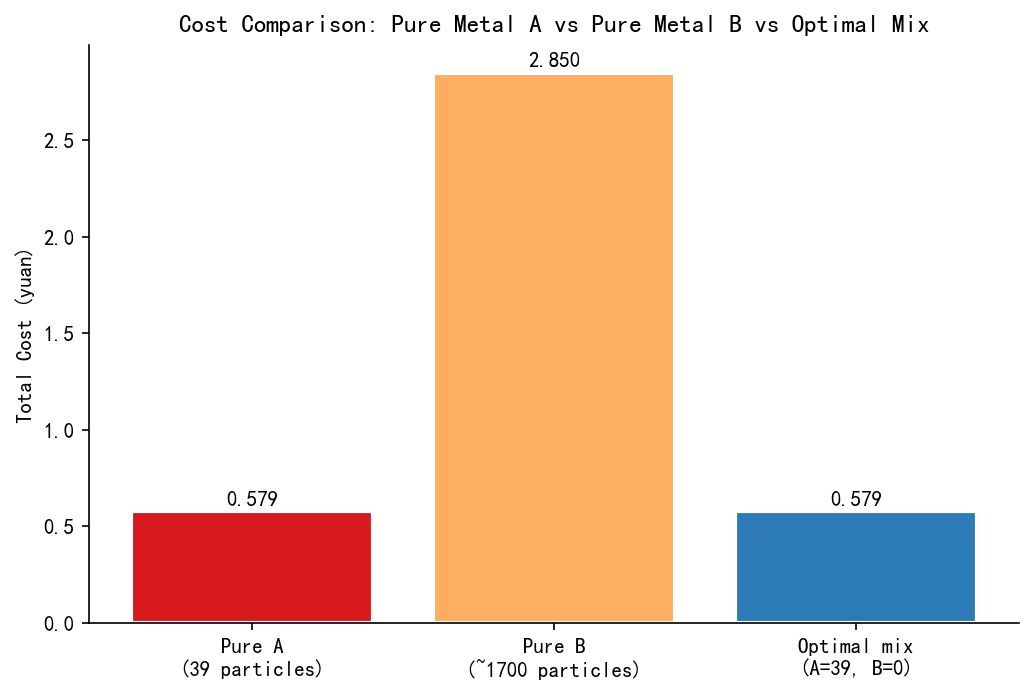
\includegraphics[width=0.8\textwidth]{../求解/问题四/图片/成本对比图.png}
  \caption{纯金属A与最优混合方案成本对比}
  \label{fig:q4_cost}
\end{figure}

\begin{figure}[ht]
  \centering
  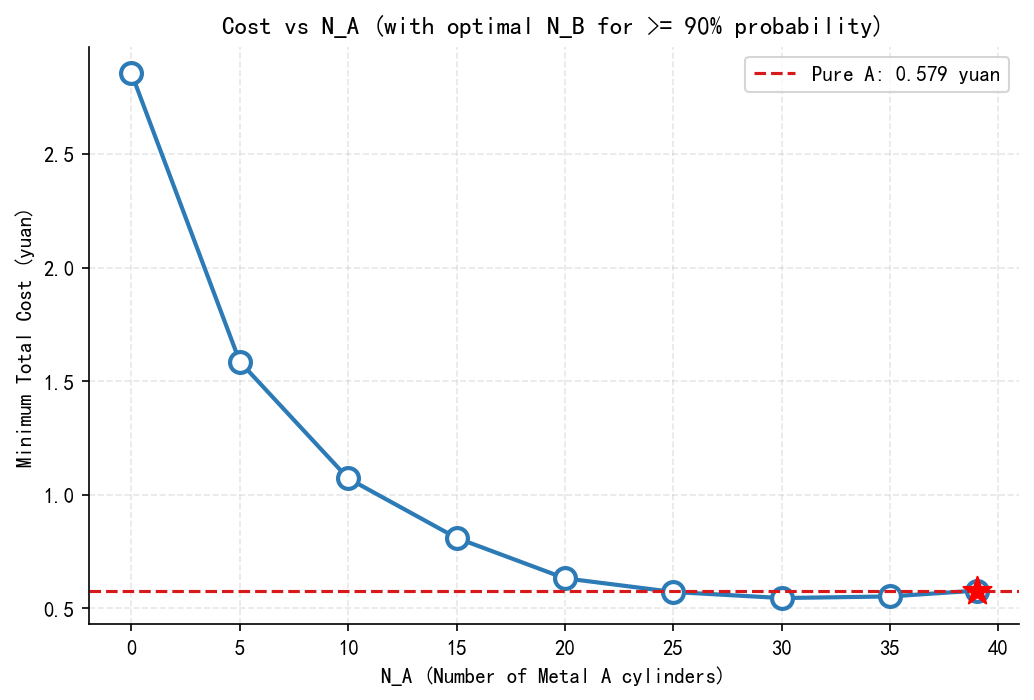
\includegraphics[width=0.8\textwidth]{../求解/问题四/图片/成本优化曲线.png}
  \caption{不同$N_A$下的最低总成本}
  \label{fig:q4_curve}
\end{figure}

优化结果汇总如表\ref{tab:问题四结果}所示。

\begin{longtable}{>{\centering\arraybackslash}p{0.14\textwidth}>{\centering\arraybackslash}p{0.14\textwidth}>{\centering\arraybackslash}p{0.18\textwidth}>{\centering\arraybackslash}p{0.18\textwidth}>{\centering\arraybackslash}p{0.16\textwidth}}
  \caption{问题四优化方案对比}
  \label{tab:问题四结果} \\
  \toprule
  方案 & 颗粒数 & 总填充率 & 导通概率 & 总成本（元） \\
  \midrule
  \endfirsthead
  \caption{问题四优化方案对比（续）} \\
  \toprule
  方案 & 颗粒数 & 总填充率 & 导通概率 & 总成本（元） \\
  \midrule
  \endhead
  \bottomrule
  \endfoot
  纯金属A & $N_A=39$ & 0.0551\% & 0.9060 & 0.579 \\
  纯金属B & $N_B\approx1700$ & $\approx$5.70\% & $\approx$0.90 & $\approx$2.85 \\
  最优方案 & $N_A=39$, $N_B=0$ & 0.0551\% & 0.9060 & 0.579 \\
\end{longtable}

由表\ref{tab:问题四结果}可知，最优方案为纯金属A方案：$N_A=39$，$N_B=0$，总成本0.579元。这一结果源于金属A圆柱体极高的长径比（83:1）带来的超低渗透阈值（0.0551\%），使得即使金属B的单颗粒成本仅为金属A的11.3\%，也无法通过混合方案降低总成本。

综上所述，问题四确定的最优配置为仅使用39个金属A圆柱体，成本0.579元。该结果揭示了在导电复合材料设计中，填料几何形状（高长径比）对经济性的决定性影响远大于材料本身的价格差异。
